\documentclass[11pt]{article}
\usepackage{fullpage}
\usepackage{graphicx}
\usepackage{enumitem}

\title{CS63 Spring 2024\\Final Project Checkpoint}
\author{Kanyarin Boonkongchuen, Mark Lohatepanont, Rachel Sun}
\date{}

\begin{document}

\maketitle

\section{Project Goal}

% This section should contain a brief overview of the primary goal of your
% project.

Using AI methods: Reinforcement Learning (RL) and A Star (A*) search, to explore how to solve a maze problem similar to that of lab 1's. 
We want to compare if there is a significant difference between the performance of these two techniques and also how the implementation differs between these two techniques.

\section{AI Methods Used}

% This section should clearly list and describe the different AI algorithms,
% techniques, and/or methods you plan to use for your project.

External Tools:\\
\indent ATIK library (Backup)\\
\indent  10 500x500 Pixel maps png format (Drawn artfully in pain)\\

\begin{figure}
  \centering
  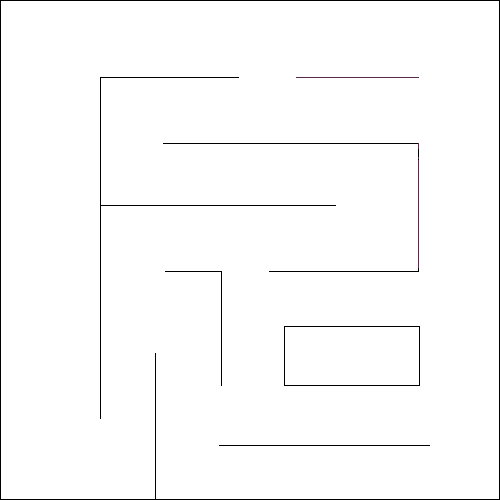
\includegraphics[totalheight=8cm]{Maps/Maze1.png}
      \caption{Example of Map}
  \centering
\end{figure}

\noindent
Packages:\\
\indent Keras\\
\indent Numpy\\
\indent Cv2 (Graphical Rendering)\\
\indent Matplotlb\\


\noindent
Algorithms:\\
\indent Reinforcement Learning via Approximate Q algorithm\\
\indent A* State Space Search\\

\section{Staged Development Plan}

% This section should contain an ordered list of sub-goals you can use as
% incremental targets on your way to your overall goal, as well as ``stretch
% goals'' to pursue after achieving your primary goal.

% Because it is often hard to estimate the difficulty of AI problems, it
% is important to have a staged plan that allows you to adapt if things
% go faster or slower than you expect.  For this reason, it's best to
% design your sub-goals and stretch-goals such that any one could
% concievably be used as a basis for a final report/presentation if
% necessary; then, try to get as far as you can in the time available.

Week 1
\begin{itemize}[noitemsep]
  \item Make maps
  \item Make an Environment
  \item Implement A* for search task
\end{itemize}
\noindent
Week 2
\begin{itemize}[noitemsep]
    \item Finish implementing A*
    \item Test A*
    \item Implement RL
\end{itemize}
\noindent
Week 3
\begin{itemize}[noitemsep]
    \item Finish implementing RL
    \item Test RL
    \item Compare results
    \item Write paper
\end{itemize}

\section{Measure of Success}

% This section should describe what ``success'' looks like for your
% project, and how you will measure progress towards that goal.

Our main goal, is to successfully implement our own environment and build a A*
and RL algorithm that is able to solve a maze. Our measure of success in
developing these two algorithms will be its capabilities to explore and solve
the 10 maps we created without any prior knowledge of any of the maps.
\\
\\
Our subgoals would be to see if A* and RL is able to generate suitable and optimal policy through the maze. 
Even if we are unable to actuate the robot, a optimal policy which the robot theoretically can navigate will still be usefull. 

\section{Plans for Analyzing Results}

% This section should describe what experimental and statistical methods
% you will use to analyze and validate your results.

Quantitatively, we can explore which of the two algorithms perform their maze searching prowess 
in faster time. A faster algorithm should indicate better performance. We can also explore things 
such as states searched, nodes explored and training time. While RL may theoretically find an optimal
solution it doesn't have the same garuntees as A* to converge on an optimal solution. So each method 
may have different pros and cons that we want to compare. Also we want want to compare our implementations
of these methods and how they compare to the theoretical benefits of each algorithm. 



\end{document}
